\documentclass{standalone}
\usepackage[margin=1in,vmargin=1in]{geometry}
\usepackage{tikz}
\usepackage{graphicx}

\begin{document}
\newcommand\myopacity{0.4}
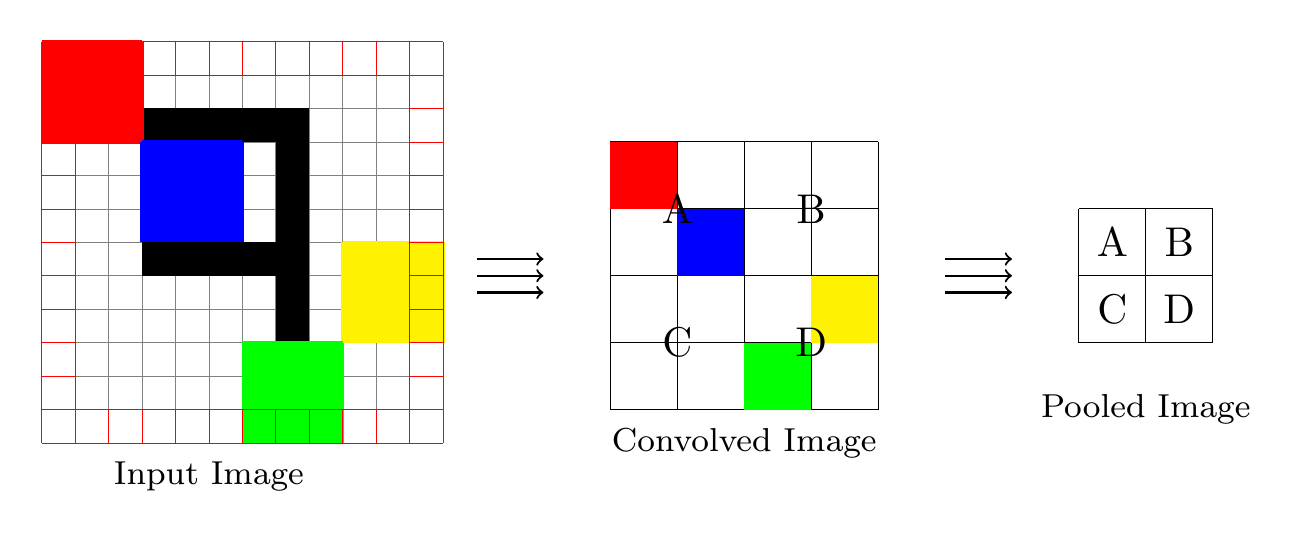
\begin{tikzpicture}[thick,scale=0.85, every node/.style={scale=1.5}]
  % -=-=-=- ADDING ZEROS -=-=-=-
  % \addNumbersConv
  \node (input) at (2,-1) {\footnotesize Input Image};
  \node (input) at (10,-0.5) {\footnotesize Convolved Image};
  \node (input) at (16,0) {\footnotesize Pooled Image};

  % -=-=-=-=- REST OF IMAGE -=-=-=-=-
  \node (A) at (0,0) {};
  \node (B) at (5,5) {};

  \node (bA) at (3.5,4.5) {};
  \node (bB) at (3,0.5) {};

  \node (bC) at (1,4.5) {};
  \node (bD) at (3,4) {};

  \node (bE) at (1,4) {};
  \node (bF) at (1.5,2.5) {};

  \node (bG) at (1,2.5) {};
  \node (bH) at (3,2) {};

  \draw[step=0.5cm,gray,very thin] (A) grid (B);
  
  \fill[black,opacity=\myopacity] (bA) rectangle (bB) {};
  \fill[black,opacity=\myopacity] (bC) rectangle (bD) {};
  \fill[black,opacity=\myopacity] (bE) rectangle (bF) {};
  \fill[black,opacity=\myopacity] (bG) rectangle (bH) {};

  % -=-=-=-=- CONVOLUTION IMAGE PORTION -=-=-=-=-=-
  \node (cA) at (-0.5,4) {};
  \node (cB) at (1,5.5) {};
  \draw[step=0.5cm,red,very thick,xshift=0cm,yshift=4cm] (cA) grid (cB);
  \fill[red,opacity = \myopacity] (cA) rectangle (cB) {};

  \node (cA) at (1,2.5) {};
  \node (cB) at (2.5,4) {};
  \draw[step=0.5cm,blue,very thick,xshift=1cm,yshift=4cm] (cA) grid (cB);
  \fill[blue,opacity = \myopacity] (cA) rectangle (cB) {};

  \node (cA) at (4,1) {};
  \node (cB) at (5.5,2.5) {};
  \draw[step=0.5cm,yellow,very thick,xshift=4cm,yshift=4cm] (cA) grid (cB);
  \fill[yellow,opacity = 0.4] (cA) rectangle (cB) {};

  \node (cA) at (2.5,-0.5) {};
  \node (cB) at (4,1) {};
  \draw[step=0.5cm,green,very thick,xshift=3cm,yshift=4cm] (cA) grid (cB);
  \fill[green,opacity = 0.4] (cA) rectangle (cB) {};

  % -=-=-=-=- ZERO PADDING -=-=-=-=-
  \node (dA) at (-0.5,5) {};
  \node (dB) at (5.5,5.5) {};
  \node (dC) at (5,-0.5) {};
  \node (dD) at (5.5,5.5) {};
  \draw[step=0.5cm,red, very thin,xshift=0cm,yshift=0cm] (-0.5,-0.5) grid (5.5,0);
  \draw[step=0.5cm,red, very thin,xshift=0cm,yshift=0cm] (-0.5,0) grid (0,5.5);
  \draw[step=0.5cm,red, very thin,xshift=4cm,yshift=0cm] (dC) grid (dD);
  \draw[step=0.5cm,red, very thin,xshift=0cm,yshift=3cm] (dA) grid (dB);
  % -=-=-=-=-= ARROWS OF DIRECTIONS
  \draw[thick,black,->] (6,2.25) --(7,2.25) {};
  \draw[thick,black,->] (6,2) --(7,2) {};
  \draw[thick,black,->] (6,1.75) --(7,1.75) {};

  \draw[thick,black,->] (13,2.25) --(14,2.25) {};
  \draw[thick,black,->] (13,2) --(14,2) {};
  \draw[thick,black,->] (13,1.75) --(14,1.75) {};


  % -=-=-=-=- RESULTING IMAGE -=-=-=-=-
  \node (A) at (8,0) {};
  \node (B) at (12,4) {};
  \draw[black,thin] (8,0) -- (8,4);
  \draw[step=1cm,black,thin] (A) grid (B);
  \fill[red,opacity=\myopacity] (8,3) rectangle (9,4) {};
  \fill[blue,opacity=\myopacity] (9,2) rectangle (10,3) {};
  \fill[yellow,opacity=\myopacity] (11,1) rectangle (12,2) {};
  \fill[green,opacity=\myopacity] (10,0) rectangle (11,1) {};

  % -=-=-=--=- POOLING IMAGE -=-=-=-=-
  \node (pA) at (9,3) {A};
  \node (pB) at (11,3) {B};
  \node (pC) at (9,1) {C};
  \node (pD) at (11,1) {D};

  \node (pW) at (15.5,2.5) {A};
  \node (pX) at (16.5,2.5) {B};
  \node (pY) at (15.5,1.5) {C};
  \node (pZ) at (16.5,1.5) {D};


  \node (pE) at (15,1) {};
  \node (pF) at (17,3) {};

  \draw[black,thin] (15,1) -- (15,3);
  \draw[black,thin] (15,1) -- (17,1);
  \draw[black,thin] (17,3) -- (17,1);
  \draw[step=1cm,black,thin] (pE) grid (pF);

\end{tikzpicture}
\end{document}